% Options for packages loaded elsewhere
\PassOptionsToPackage{unicode}{hyperref}
\PassOptionsToPackage{hyphens}{url}
%
\documentclass[10pt,a4paper]{article}
\usepackage[left=25mm,right=25mm]{geometry}
\usepackage{amsmath}
\usepackage{amsfonts}
\usepackage{amssymb}

\author{}
\date{}



\usepackage{listings}
\usepackage{color}

\definecolor{dkgreen}{rgb}{0,0.6,0}
\definecolor{gray}{rgb}{0.5,0.5,0.5}
\definecolor{mauve}{rgb}{0.58,0,0.82}

\lstset{frame=tb,
  language=C,
  aboveskip=3mm,
  belowskip=3mm,
  showstringspaces=false,
  columns=flexible,
  basicstyle={\small\ttfamily},
  numbers=none,
  numberstyle=\tiny\color{gray},
  keywordstyle=\color{blue},
  commentstyle=\color{dkgreen},
  stringstyle=\color{mauve},
  breaklines=true,
  breakatwhitespace=true,
  tabsize=3
}

\usepackage{multicol}
\usepackage{graphicx}
\usepackage{epstopdf}

\epstopdfDeclareGraphicsRule{.gif}{png}{.png}{convert gif:#1 png:\OutputFile}
\AppendGraphicsExtensions{.gif}
\usepackage{chngcntr}
\counterwithin*{equation}{section}
\counterwithin*{equation}{subsection}
\usepackage{amsmath}

\usepackage{float} 
\usepackage{hyperref}
\usepackage{amsmath}
\let\oldsubsection\subsection
\renewcommand{\subsection}{%
    \setcounter{equation}{0}%
    \oldsubsection%
}
\begin{document}


\begin{flushleft}
\begin{LARGE}EE 435 Homework 4 Spring 2024
\end{LARGE}
\\Jonathan Hess
\\\href{https://github.com/Jetsama/EE435/tree/main/HW4}{GitHub Page}
\end{flushleft}


\subsection*{Problem 1 and 2}
The model parameters $\mu$, C OX, VTH and $\lambda$ are widely used in analytical
formulations of the performance of analog circuits. These parameters are used to
characterize how MOS transistors operate in the square-law model of the transistor.
When operating in the saturation region, the square-law model for the drain
current of transistors can be expressed as
$I_D =  $


Though this square-law formulation is a simplification, it gives reasonable results that
can be used for much of the design process. Better and more comprehensive models,
such as the BSIM models, are then used in computer simulations to more accurately
predict performance and for refining the design to meet target specifications. The BSIM
models, however, are not analytically tractable and thus unsuitable for analytical
formulations. Though intermediate models that are more accurate than the square-law
models and less comprehensive than the BSIM models exist, there is little evidence of
analytical tractability for models with complexity beyond that of the square-law model.
Many analog circuits are quite sensitive to the parameter $\lambda$ in the square-law
model. Unfortunately, the parameter $\lambda$ is quite sensitive to device dimensions and
operating point. As such, a table or plot of $\lambda$ parameters is useful when using the square-
law model for predicting the performance of many analog circuits based upon the square-
law model.
Generate plots of $\lambda$ for both n-channel and p-channel transistors in the 0.18$\mu$m
CMOS for different lengths and for three different values of W and for three different
values of VDS as shown below. Comment on how $\lambda$ varies with device dimensions and
operating points. When determining $\lambda$, assume that the devices are modeled by the
BSIM model which is embedded in the PDK file used in SPECTRE. Extract $\lambda$ at a given
operating point by taking two measurements (simulation results) of the drain current at
values of VDS slightly above and slightly below the target VDS value on a constant VGS
locus as shown in the plot below. This is likely how you extracted the parameter $\lambda$ in EE
330. The length should vary between LMIN and 20LMIN and the VDS values should be
from slightly above VEB to 2.5V.


\subsection*{Problem 3}

Consider the 5T op amp configured used as a transconductance amplifier
in the circuit shown below. Assume the op amp is designed in a 0.18$\mu$m ON CMOS
process with VDD =1.2V, VSS=-1.2V, L=2$\mu$m and V EB=100mV for all transistors, and the
power in the op amp is 1mW. Assume $\lambda$=.01V

\subsubsection*{a)}What is W1?\\
\\
To find all W we can look at constraints.\\
$W1 = W2$\\
$W3 = W4$\\
$P = 2.4V (Id) = 1mW$\\
$V_{EB} = 100mV = VGS-Vt$\\
$V_{SD3} + V_{DS1} + V_{DS5} = 2.4$
\\
The max tail current is 416.6$\mu$A which means that current through M1 is 208.3$\mu$A. Using the current equation and K from the datasheet (K = 171.8$\mu$)we get:\\
$I_d = \frac{W}{L}(K)(VGS-Vt)^2(1+V_{DS}\lambda) = 208.3\mu A = (.01)* 171.8\mu * \frac{W}{L}(1+V_{DS}(.01))$\\
$I_d = \frac{W}{L}(K)(VGS-Vt)^2= 208.3\mu A = (.01)* 171.8\mu * \frac{W}{L}$\\
We get that:\\
$w = 121.265 * L = 242.53\mu m$\\ 


\subsubsection*{b)} What is the quiescent voltage at the source of M1 ?\\
\\
The voltage drop across M3 is id*Gm3
The voltage on source

\subsubsection*{c)}Obtain an expression for the small signal voltage gain of the OTA circuit in terms of the small-signal parameters g m1, R1 , and C1.

These expressions are available in the lecture 5 slides\\
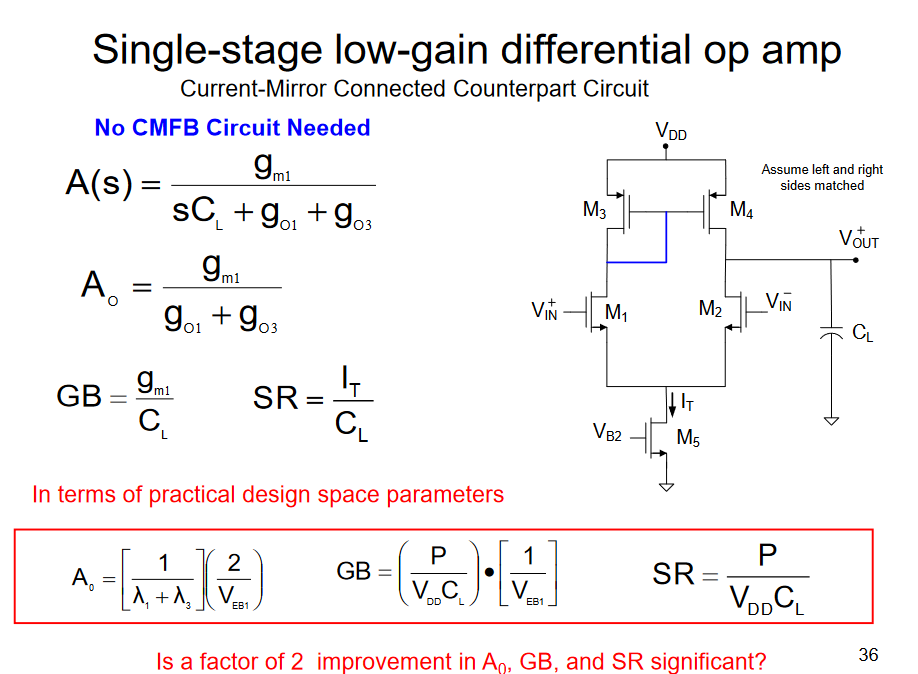
\includegraphics[width=3in]{images/Lecture5Slide.png} \\

These were found by splitting the circuit into quarters and mirroring the left and right sides.\\
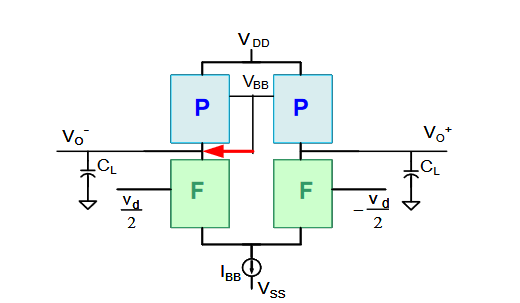
\includegraphics[width=3in]{images/Mirror.png} \\
By doing this we can analyze the F and P circuits individually.\\
\\
For the P circuit we have a single transistor connected to itself. Because of the current mirror the second P (on the right side) is also virtually connected to itself. This means that it acts as a resistor with no external biasing.\\
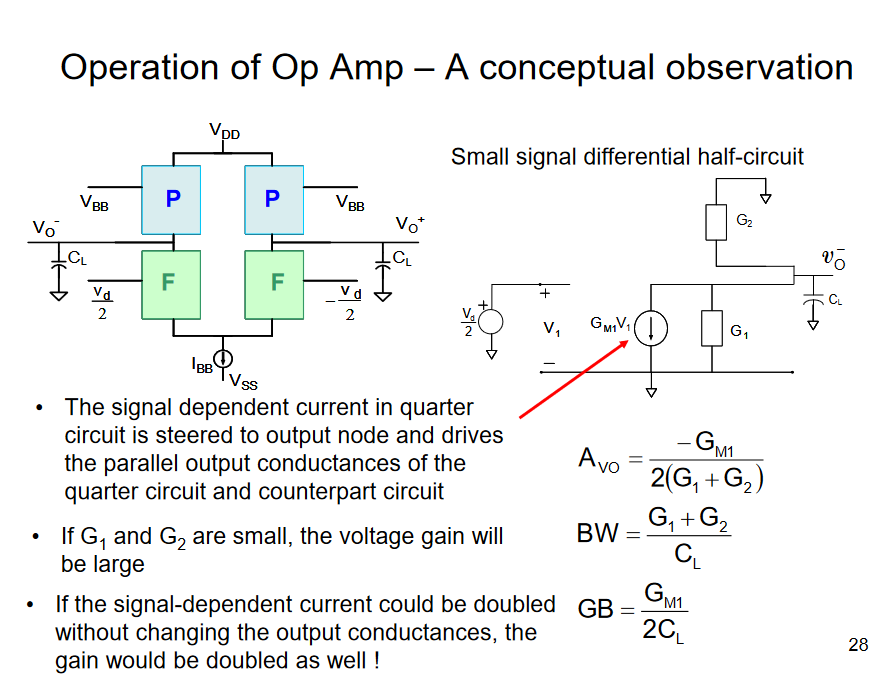
\includegraphics[width=3in]{images/Lecture5Slide28.png} \\

\subsubsection*{d)}Numerically determine and plot the small signal frequency dependent voltage gain if R1 =50K and C1 =40pF\\

\subsubsection*{e)}Determine the 3dB bandwidth\\

\subsubsection*{f)}How does the 3dB bandwidth change if the power in increased by 20\% by changing VB2?\\


http://class.ece.iastate.edu/ee435/miscHandouts/TSMC%200.18%20T48K.pdf

http://class.ece.iastate.edu/ee330/lectures/EE%20330%20Lect%2025%20Fall%202023.pdf

\end{document}







